% This work is made available under the terms of the
% Creative Commons Attribution-ShareAlike 4.0 license,
% http://creativecommons.org/licenses/by-sa/4.0/.

\documentclass[a4paper]{book}

\usepackage{wrapfig}
\usepackage{graphicx}
\usepackage{hyperref}
\usepackage{multirow}
\usepackage{scalefnt}
\usepackage{tikz}
\usepackage{varwidth}

% watermark -- for draft stage
%\usepackage[firstpage]{draftwatermark}
%\SetWatermarkLightness{0.9}
%\SetWatermarkScale{5}

\hyphenation{ImageMagick}
\hyphenation{ImageJ}

% Copyright (c) 2009 by the University of Waikato, Hamilton, NZ. 
% This work is made available under the terms of the 
% Creative Commons Attribution-ShareAlike 3.0 license, 
% http://creativecommons.org/licenses/by-sa/3.0/. 
%
% Version: $Revision$

\newenvironment{tight_itemize}{
\begin{itemize}
  \setlength{\itemsep}{1pt}
  \setlength{\parskip}{0pt}
  \setlength{\parsep}{0pt}}{\end{itemize}
}

\newenvironment{tight_enumerate}{
\begin{enumerate}
  \setlength{\itemsep}{1pt}
  \setlength{\parskip}{0pt}
  \setlength{\parsep}{0pt}}{\end{enumerate}
}

% if you just need a simple heading
% Usage:
%   \heading{the text of the heading}
\newcommand{\heading}[1]{
  \vspace{0.3cm} \noindent \textbf{#1} \newline
}

\newcommand{\icon}[1]{\tikz[baseline=-3pt]\node[inner sep=0pt,outer sep=0pt]{\includegraphics[height=1.1em]{#1}};}


\title{
  \textbf{ADAMS} \\
  {\Large \textbf{A}dvanced \textbf{D}ata mining \textbf{A}nd \textbf{M}achine
  learning \textbf{S}ystem} \\
  {\Large Module: adams-imaging} \\
  \vspace{1cm}
  
\includegraphics[width=2cm]{images/imaging-module.png} \\
}
\author{
  Peter Reutemann
}

\setcounter{secnumdepth}{3}
\setcounter{tocdepth}{3}

\begin{document}

\begin{titlepage}
\maketitle

\thispagestyle{empty}
\center
\begin{table}[b]
	\begin{tabular}{c l l}
		\parbox[c][2cm]{2cm}{\copyright 2009-2022} &
		\parbox[c][2cm]{5cm}{
\includegraphics[width=5cm]{images/coat_of_arms.pdf}} \\
	\end{tabular}
	
\includegraphics[width=12cm]{images/cc.png} \\
\end{table}

\end{titlepage}

\tableofcontents
\listoffigures
%\listoftables


%%%%%%%%%%%%%%%%%%%%%%%%%%%%%%%%%%%
\chapter{ADAMS}
ADAMS has custom image processing support that does not rely on other libraries.

The following actors are available:
\begin{tight_itemize}
	\item \texttt{sink.ImageFileWriter} -- writes an image container to a file
	using the specified writer.
	\item \texttt{transformer.BufferedImageTransformer} -- performs a transformation
	using an existing transformer class on the incoming image and
	outputs another image again.
	\item \texttt{transformer.BufferedImageFeatureGenerator} -- turns a
	\texttt{BufferedImageContainer} into an \texttt{weka.core.Instance} object to
	be used in WEKA. The attaced meta-data in form of a report can be added to the
	output object as well.
	\item \texttt{transformer.ImageFileReader} -- reads an image file using the
	specified image reader.
\end{tight_itemize}

Figure \ref{adams-blur-flow} shows a
flow\footnote{adams-imaging-gaussian\_blur.flow} for reading images, blurring
them using a gaussian blur transformer and displaying them side-by-side. Figures
\ref{adams-blur-output-original} and \ref{adams-blur-output-blurred} show original
and blurred image.

\begin{figure}[htb]
  \centering
  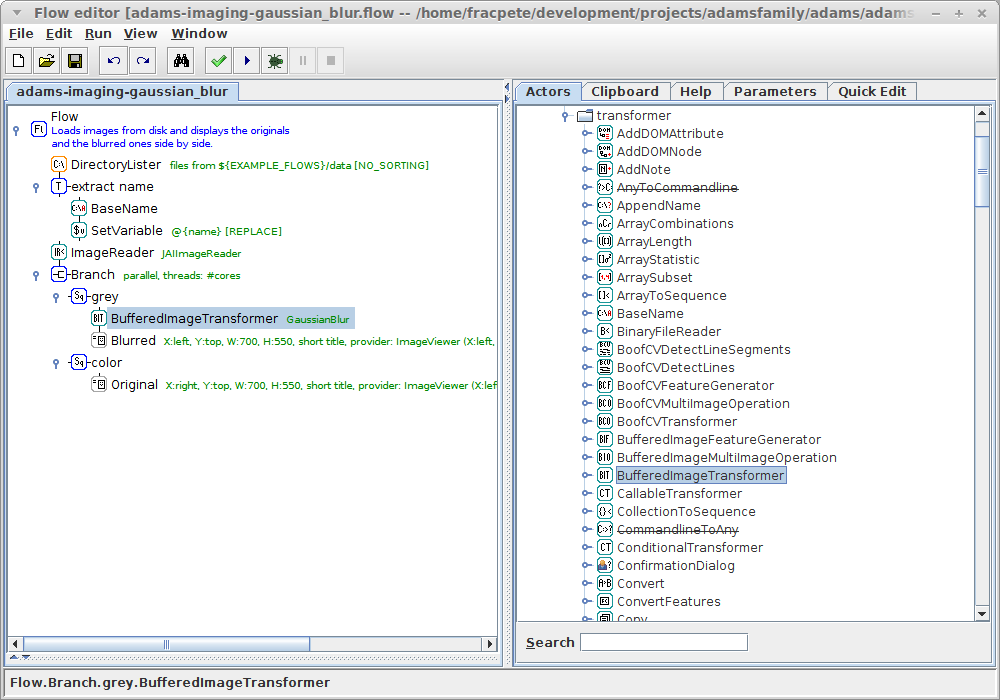
\includegraphics[width=10.0cm]{images/adams-blur-flow.png}
  \caption{Flow for blurring images stored in a directory.}
  \label{adams-blur-flow}
\end{figure}

\begin{figure}[htb]
  \begin{minipage}[b]{0.48\linewidth}
  \centering
  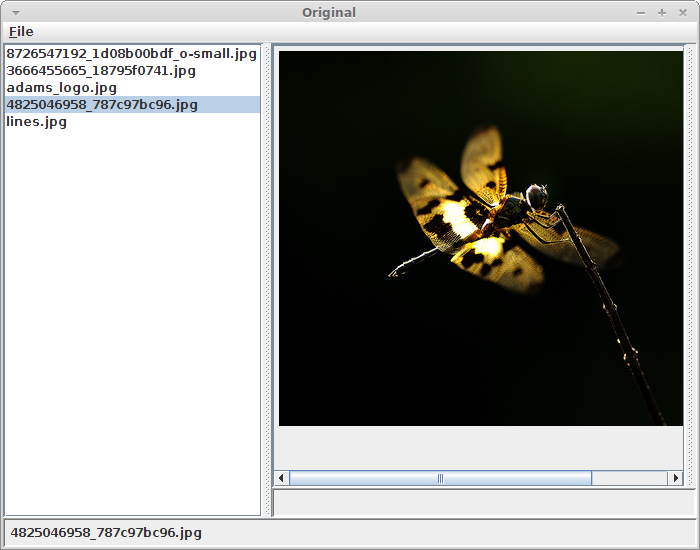
\includegraphics[height=3.7cm]{images/adams-blur-output-original.png}
  \caption{The original image.}
  \label{adams-blur-output-original}
  \end{minipage}%
  \begin{minipage}[b]{0.48\linewidth}
  \centering
  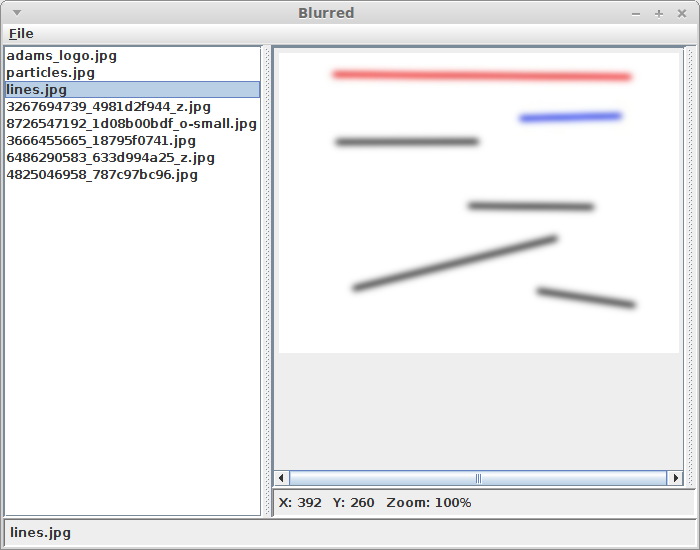
\includegraphics[height=3.7cm]{images/adams-blur-output-blurred.png}
  \caption{The blurred image.}
  \label{adams-blur-output-blurred}
  \end{minipage}
\end{figure}



%%%%%%%%%%%%%%%%%%%%%%%%%%%%%%%%%%%
\chapter[Java Advanced
Imaging]{\parbox[b]{1.2cm}{
\includegraphics[width=1cm]{images/jai.png}}\parbox[c]{14cm}{Java
Advanced Imaging}}
Java Advanced Imaging (JAI) is an API to provide a simple, high-level
programming model which allows developers to create their own image manipulation
routines\footnote{\url{http://en.wikipedia.org/wiki/Java_Advanced_Imaging}{}}.

Reading and writing images are done using the \textit{ImageFileReader} transformer
and \textit{ImageFileWriter} sink:
\begin{tight_itemize}
	\item \texttt{ImageFileReader} -- use the \textit{JAIImageFileReader}
	\item \texttt{ImageFileWriter} -- use the \textit{JAIImageFileWriter}
\end{tight_itemize}

Since the JAI actors, readers and writers use \texttt{BufferedImageContainer}, the 
\texttt{BufferedImageTransformer} and \texttt{BufferedImageFeatureGenerator}
transformers can be used.

%%%%%%%%%%%%%%%%%%%%%%%%%%%%%%%%%%%
\chapter{LIRE}
The Lucene Image Retrieval library \cite{lire} provides a wide range of feature
generators that work on \textit{BufferedImageContainer} objects:
\begin{tight_itemize}
  \item AutoColorCorrelogram
  \item BasicFeatures
  \item BinaryPatternsPyramid
  \item CEDD
  \item ColorLayout
  \item EdgeHistogram
  \item FCTH
  \item FuzzyColorHistogram
  \item FuzzyOpponentHistogram
  \item Gabor
  \item JCD
  \item JpegCoefficientHistogram
  \item LocalBinaryPatterns
  \item LuminanceLayout
  \item OpponentHistogram
  \item PHOG
  \item RotationInvariantLocalBinaryPatterns
  \item ScalableColor
  \item SimpleColorHistogram
  \item Tamura
\end{tight_itemize}


%%%%%%%%%%%%%%%%%%%%%%%%%%%%%%%%%%%
\chapter{Object conversion}
The following conversions are available:
\begin{tight_itemize}
  \item \textit{ColorToHex} -- turns a Color into its hexa-decimal
  notation.
  \item \textit{HexToColor} -- turns a color in hexa-decimal notation back
  into a Color object.
  \item \textit{LocatedObjectToRectangle} -- extracts the location of the
  object and stores it in a rectangle object.
  \item \textit{ObjectAnnotationsToImageSegmentationLayers} -- converts the
  object annotations into layers for image segmentation.
  \item \textit{QuadrilateralLocationCenter} -- outputs the center of the
  QuadrilateralLocation object.
  \item \textit{QuadrilateralLocationToString} -- turns the
  QuadrilateralLocation object into its string representation.
  \item \textit{RectangleCenter} -- outputs the center of the rectangle object.
  \item \textit{RectangleToString} -- converts the rectangle object into its
  string representation.
  \item \textit{StringToQuadrilateralLocation} -- creates a QuadrilateralLocation
  object from this string representation.
  \item \textit{StringToRectangle} -- creates a rectangle object from the string
  representation.
\end{tight_itemize}


%%%%%%%%%%%%%%%%%%%%%%%%%%%%%%%%%%%
\chapter{OCR}
A common task in image processing is \textit{optical character recognition} 
(OCR). ADAMS offers a simple wrapper around the open-source \textit{tesseract} 
engine \cite{tesseract}. The engine is available for Windows, Linux and Mac OSX.
It supports multiple languages, however, these need to be installed in order to
be actually available.

The follwoing actors are available:
\begin{tight_itemize}
	\item \textit{TesseractConfiguration} -- standalone for configuring OCR, 
	mainly to define where the tesseract executable is located.
	\item \textit{TesseractOCR} -- this transformer turns an image file into
	one or more text files, which need to be further processed in the flow
	then.\footnote{adams-imaging-ocr.flow}
\end{tight_itemize}

By default, the \textit{TesseractConfiguration} standalone uses the globally
defined preferences as default values. In the preferences dialog 
(\textit{Main menu $\rightarrow$ Program $\rightarrow$ Preferences 
$\rightarrow$ Tesseract}) you can specify the location of the tesseract
executable and the default language (see Figure \ref{tesseract-preferences}).
\begin{figure}[htb]
  \centering
  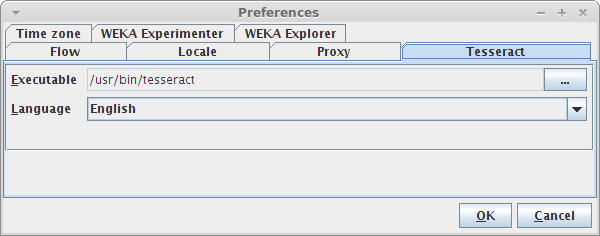
\includegraphics[width=10.0cm]{images/tesseract-preferences.png}
  \caption{Preferences for tesseract.}
  \label{tesseract-preferences}
\end{figure}


%%%%%%%%%%%%%%%%%%%%%%%%%%%%%%%%%%%
\chapter{Interaction}
The \textit{PixelSelector} transformer allows the user to interact with the
flow. The interaction with the user works as follows: an image viewer instance
is displayed when the \textit{PixelSelector} transformer receives an image token
as input. The use then right-clicks on a pixel that he wants to process, e.g.,
labelling for WEKA data generation. After all the pixels have been selected and
processed, the user then hits the \textit{OK} button to close the dialog. The
\textit{PixelSelector} then forwards the image container with the
attached, enriched report for further processing.

The \textit{PixelSelector} transformer is very generic, which means the actor
is responsible for the actions that the user can select from the right-click
menu. This is done by selecting the appropriate actions from the list of
available ones, e.g., \textit{AddClassification} (package
\texttt{adams.flow.transformer.pixelselector}), which is used for attaching
classification labels to pixels. In order to make these selections visible not
just in the report that is displayed on the right-hand side in the dialog,
appropriate overlays can be selected as well, e.g., the
\textit{ClassificationOverlay} (package
\texttt{adams.flow.transformer.pixelselector}) overlay, which displays the
pixels with the associated labels on the screen.

Figure \ref{pixelselector-flow} shows a
flow\footnote{adams-imaging-pixelselector.flow} that lets the user hand-label
all JPG images in a directory and generated WEKA data from it. It uses a cropped
region of 5x5 pixels around the selected pixels for the data generation. The
user interface for selecting the pixels is shown in Figure
\ref{pixelselector-interaction} and a resulting dataset in Figure
\ref{pixelselector-dataset}.

\begin{figure}[htb]
  \centering
  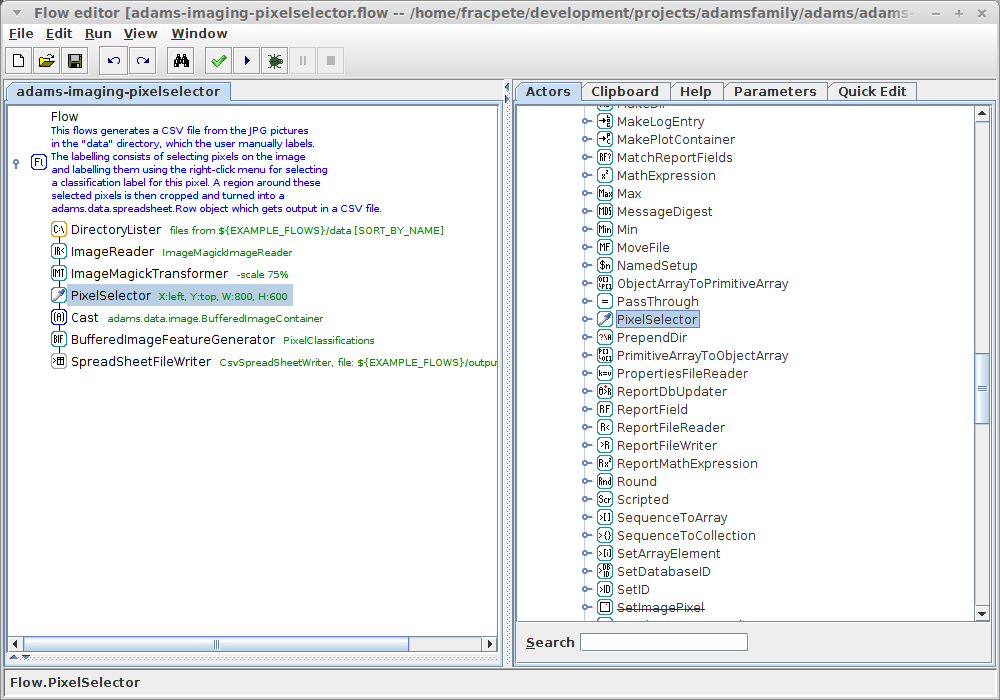
\includegraphics[width=10.0cm]{images/pixelselector-flow.png}
  \caption{Flow for generating ARFF file from user-labelled pixels.}
  \label{pixelselector-flow}
\end{figure}

\begin{figure}[htb]
  \centering
  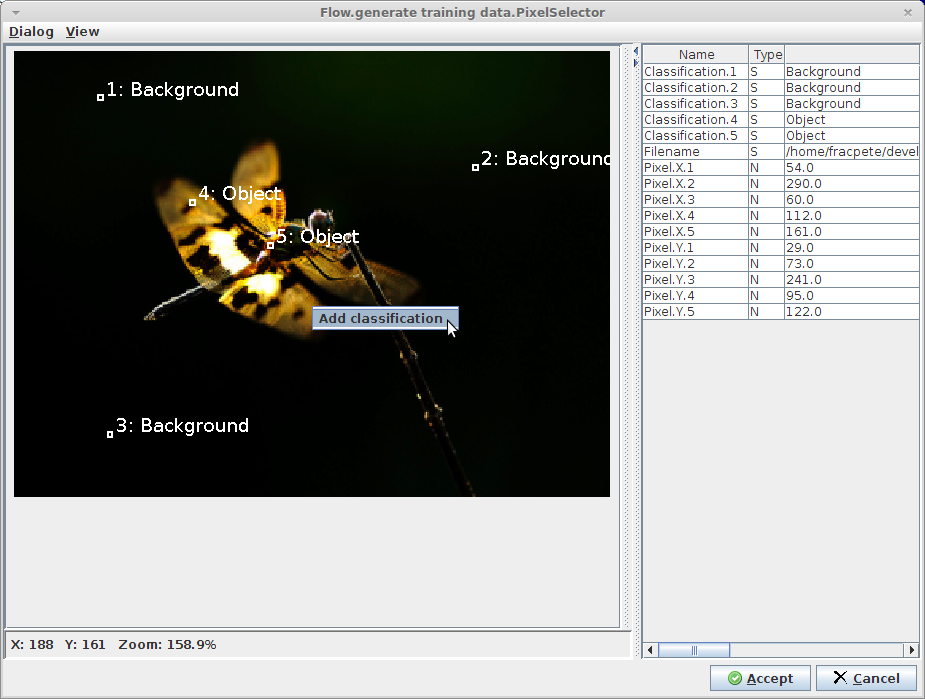
\includegraphics[width=10.0cm]{images/pixelselector-interaction.png}
  \caption{User interface for labelling pixels, displaying some pixels
  labelled already.}
  \label{pixelselector-interaction}
\end{figure}

\begin{figure}[htb]
  \centering
  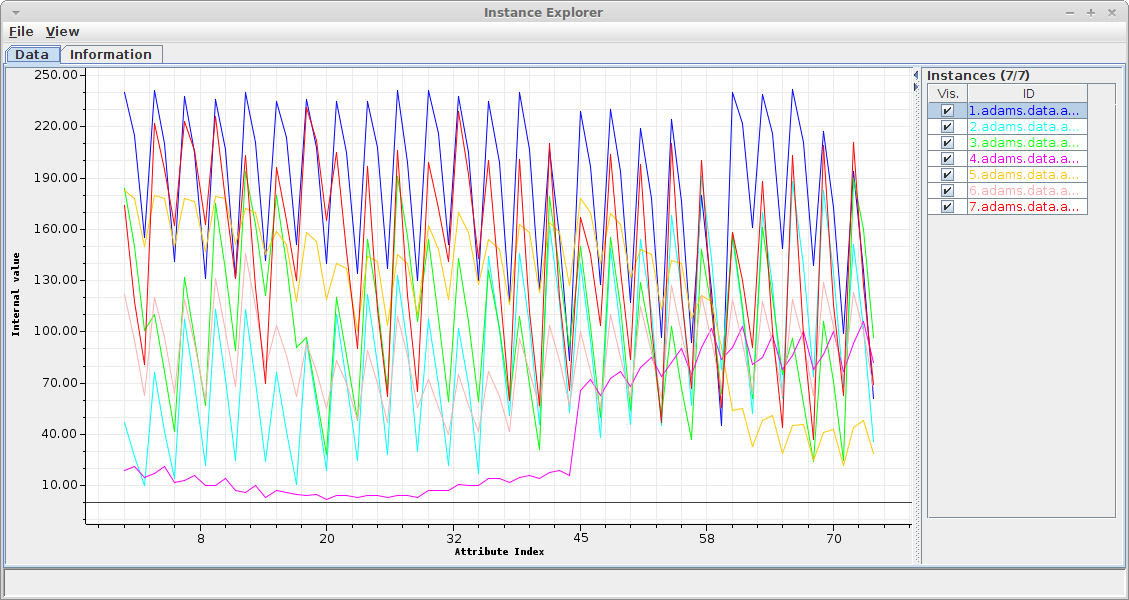
\includegraphics[width=10.0cm]{images/pixelselector-dataset.png}
  \caption{Example dataset generated using the PixelSelector.}
  \label{pixelselector-dataset}
\end{figure}

Of course, due to the interactive nature, labelling is performed on-the-fly and
no record is kept. Once the image has been processed, the
\textit{PixelSelector} will forget about it. If you want to preserve the
attached report, you can use the \textit{ReportFileWriter} transformer to save
the report to disk. 

In order to re-use a previously saved report, you can use the
\textit{SetReportFromFile} or \textit{SetReportFromSource} transformer to
replace the default report in the image container after you loaded the image
with the one stored on disk. This allows you to continue work with previously
generated labels, saving you a lot of work.

Since the \textit{SetReportFromFile} and \textit{SetReportFromSource}
transformers generate \textit{ReportHandler} tokens, you need to explicitly
cast the type of the tokens to the desired one, e.g.,
\textit{BufferedImageContainer}, using the \textit{Cast} control actor.

% %%%%%%%%%%%%%%%%%%%%%%%%%%%%%%%%%%
\chapter{Feature output}
Of course, the data can be turned into a format that is suitable for machine 
learning applications like WEKA (\cite{weka}). For JAI transformer tokens, the
\textit{BufferedImageFeatureGenerator} can be used to generate such output.

%%%%%%%%%%%%%%%%%%%%%%%%%%%%%%%%%%%
\chapter{Miscellaneous flow components}
The imaging module offers some more actors that have not been introduced yet.

\noindent Available conditions:
\begin{tight_itemize}
  \item \textit{HasExifTag} -- checks whether the specified tag is present in
  the data coming through.
\end{tight_itemize}

\noindent Available sources:
\begin{tight_itemize}
  \item \textit{ColorProvider} -- outputs Color objects generated by a
  configured color provider.
  \item \texttt{NewImage} -- creates an image with a specific color and
  user-defined dimensions.
\end{tight_itemize}

\noindent Available transformers:
\begin{tight_itemize}
  \item \textit{ChangeImageObjectPrefix} -- replaces the prefix of
  objects in a report with a new one.
  \item \textit{ColorProvider} -- outputs Color objects whenever a token
  passes through.
  \item \texttt{CompareObjectLocations} -- for visually comparing annotations
  and predicted object locations side-by-side on the same image.
  \item \textit{CountObjectsInRegion} -- counts the objects that fall
  within the defined region (partial counts possible, too).
  \item \textit{DecodeBarcode} -- allows extracting of barcodes like
  EAN and QRCode from images\footnote{adams-imaging-barcode.flow}.
  \item \texttt{DetermineOverlappingObjects} -- computes overlapping image objects
  between two reports (annotations and predictions).
  \item \textit{Draw} -- Performs draw operations on images, like setting
  pixels, drawing lines, rectangles, ovals, text, images\footnote{adams-imaging-draw.flow}
  and even barcodes (e.g., EAN and QRCode)\footnote{adams-imaging-barcode.flow}.
  \item \textit{ExifTagOperation} -- allows operations on EXIF meta-data tags.
  \item \texttt{GetImageObjectIndices} -- lists all the indices of the objects
  stored in the report, as located by the specified finder.
  \item \texttt{GetImageObjects} -- lists all the objects stored in the
  report, as located by the specified finder.
  \item \texttt{GetImageObjectMetaData} -- retrieves the meta-data of
  the located object.
  \item \textit{ImageInfo} -- Allows you to obtain \textit{width} and
  \textit{height} information from an image.
  \item \texttt{ImageLabeler} -- allows the user to interactively label/classify
  images, attaching the label to the report.
   annotate objects (i.e., attach labels) that were located in an image.
  \item \textit{ImageMetaData} -- Extracts meta-data (EXIF or IPTC) from an
  image as spreadsheet using various libraries (e.g., Sanselan\cite{sanselan},
  Meta-Data Extractor\cite{metadataextractor}).\footnote{adams-imaging-meta\_data.flow}
  \item \texttt{ImageObjectAnnotator} -- allows the user to interactively
   annotate objects (i.e., attach labels) that were located in an image.
  \item \textit{ImageObjectFilter} -- filters the objects in the meta-data of an image
  using the specified object finder and filter.
  \item \texttt{ImageObjectInfo} -- extracts information from a image object
  stored in a report.
  \item \texttt{ImageObjectIndexOffset} -- changes the index of the objects in the
  report by the specified offset.
  \item \texttt{ImageObjectOverlap} -- superceded by \textit{DetermineOverlappingObjects}.
  \item \texttt{ImageSegmentationAnnotator} -- allows the user to interactively
  annotate images for image segmentation.
  \item \texttt{ImageSegmentationContainerFilter} -- allows the user to apply a
  filter to an image segmentation container.
  \item \texttt{ImageSegmentationContainerOperation} -- allows the user to apply
  operations to image segmentation containers.
  \item \texttt{ImageSegmentationFileReader} -- for reading image segmentation file formats
  \item \textit{ImageSharpness} -- determines whether image is in focus or not.
  \item \texttt{IntersectOverUnion} -- superceded by \textit{DetermineOverlappingObjects}.
  \item \textit{LocateObjects} -- provides a framework for algorithms that
  locate objects in images.
  \item \texttt{MergeObjectLocations} -- merges objects locations
  in the current image container with the ones obtained from a report
  available from storage.
  \item \texttt{NegativeRegions} -- generates negative region objects
  for images passing through.
  \item \texttt{RemoveImageObject} -- removes the specified image object
  from the report.
  \item \textit{RemoveOverlappingImageObjects} -- for cleaning up
  overlapping objects, e.g., as post-processing from predicting bounding
  boxes.
  \item \texttt{ScaleReportObjects} -- scales the x/y and width/height
  of the objects stored in reports.
  \item \texttt{ViaAnnotations} -- turns reports into JSON annotations that
  can be used by VIA\cite{via}.
  \item \texttt{ViaAnnotationsToReports} -- turns VIA JSON annotations into
  separate reports, one per annotated image.
\end{tight_itemize}

\noindent Available sinks:
\begin{tight_itemize}
  \item \textit{ImageHistogram} -- displays the histogram of an image (gray or color).
  \item \texttt{ImageSegmentationFileWriter} -- for reading image segmentation file formats
\end{tight_itemize}

%%%%%%%%%%%%%%%%%%%%%%%%%%%%%%%%%%%
% Copyright (c) 2009-2012 by the University of Waikato, Hamilton, NZ. 
% This work is made available under the terms of the 
% Creative Commons Attribution-ShareAlike 4.0 license,
% http://creativecommons.org/licenses/by-sa/4.0/.
%
% Version: $Revision$

\begin{thebibliography}{999}
	% to make the bibliography appear in the TOC
	\addcontentsline{toc}{chapter}{Bibliography}

    % references
	\bibitem{adams}
		\textit{ADAMS} -- Advanced Data mining and Machine learning System \\
		\url{https://adams.cms.waikato.ac.nz/}{}

	\bibitem{esrigrid}
	 	\textit{Esri Grid} -- a raster GIS file format deveoped by Esri. \\
		\url{https://en.wikipedia.org/wiki/Esri\_grid}{}

	\bibitem{kml}
	 	\textit{Keyhole Markup Language} -- an XML notation for expressing
	 	geographic annotation and visualization within Internet-based,
	 	two-dimensional maps and three-dimensional Earth browsers. \\
		\url{http://en.wikipedia.org/wiki/Keyhole\_Markup\_Language}{}

	\bibitem{postgresql}
	 	\textit{PostgreSQL} -- a powerful, open source object-relational
	 	database system. \\
		\url{http://www.postgresql.org/}{}

	\bibitem{postgis}
		\textit{PostGIS} -- a spatial database extender for PostgreSQL
		object-relational database. It adds support for geographic
		objects allowing location queries to be run in SQL.  \\
		\url{http://postgis.net/}{}

	\bibitem{srid4269}
	 	\textit{SRID 4269} -- or NAD 83 (North American Datum). \\
		\url{http://spatialreference.org/ref/epsg/4269/}{}

	\bibitem{mysql}
		\textit{MySQL} -- an open-source relational database management
		system (RDBMS) \\
		\url{http://www.mysql.com/}{}

\end{thebibliography}


\end{document}
